\documentclass[border=3pt]{standalone}
\usepackage[T1]{fontenc}
\usepackage[utf8]{inputenc}
\usepackage{lmodern}
\usepackage{amsmath,amssymb}
\usepackage{xcolor}
\usepackage{tikz}
\usepackage{fontawesome5}
\usepackage{ragged2e}
\usetikzlibrary{shapes,shapes.geometric,shapes.misc,arrows.meta,positioning,
                calc,fit,backgrounds,decorations.pathreplacing,
                decorations.markings,patterns,chains}
\usetikzlibrary{decorations.pathreplacing,decorations.markings}
\definecolor{primary}{HTML}{1A5276}
\definecolor{secondary}{HTML}{2E86C1}
\definecolor{accent}{HTML}{E74C3C}
\definecolor{lightbg}{HTML}{EBF5FB}
\definecolor{defbg}{HTML}{FDF2E9}
\definecolor{greenhl}{HTML}{27AE60}
\definecolor{purplehl}{HTML}{8E44AD}
\definecolor{goldhl}{HTML}{B7950B}
\definecolor{tealhl}{HTML}{117A65}
\definecolor{codebg}{HTML}{F4F6F7}
\definecolor{neutral}{HTML}{707B7C}
\definecolor{dom1}{HTML}{1F618D}
\definecolor{dom2}{HTML}{117864}
\definecolor{dom3}{HTML}{6C3483}
\definecolor{dom4}{HTML}{922B21}
\definecolor{dom5}{HTML}{B7950B}
% --- carried over from ccna.sty so figures match the book exactly
\tikzset{
  dev/.style={rounded corners=3pt, draw=#1, fill=#1!8, text=#1!45!black,
              line width=0.9pt, minimum width=1.45cm, minimum height=1.05cm,
              align=center, font=\scriptsize\bfseries, inner sep=2pt},
  wirestyle/.style={line width=0.9pt, neutral!75},
  xconn/.style={line width=0.9pt, neutral!75, dash pattern=on 2.5pt off 2pt},
}

\newcommand{\Rtr}[3]{\node[dev=dom3] (#1) at #2 {\faIcon{route}\\#3};}
\newcommand{\Sw}[3]{\node[dev=dom2] (#1) at #2 {\faIcon{sitemap}\\#3};}
\newcommand{\Msw}[3]{\node[dev=dom3] (#1) at #2 {\faIcon{layer-group}\\#3};}
\newcommand{\Host}[3]{\node[dev=neutral] (#1) at #2 {\faIcon{desktop}\\#3};}
\newcommand{\Lap}[3]{\node[dev=neutral] (#1) at #2 {\faIcon{laptop}\\#3};}
\newcommand{\Srv}[3]{\node[dev=dom1] (#1) at #2 {\faIcon{server}\\#3};}
\newcommand{\Ap}[3]{\node[dev=dom5] (#1) at #2 {\faIcon{wifi}\\#3};}
\newcommand{\Wlc}[3]{\node[dev=dom5] (#1) at #2 {\faIcon{broadcast-tower}\\#3};}
\newcommand{\Fw}[3]{\node[dev=dom4] (#1) at #2 {\faIcon{shield-alt}\\#3};}
\newcommand{\Cld}[3]{\node[dev=neutral] (#1) at #2 {\faIcon{cloud}\\#3};}
\newcommand{\Phone}[3]{\node[dev=dom5] (#1) at #2 {\faIcon{phone-alt}\\#3};}
\newcommand{\Prn}[3]{\node[dev=neutral] (#1) at #2 {\faIcon{print}\\#3};}

% A link. The optional argument takes tikz options (e.g. xconn for a
% trunk drawn dashed); the fourth argument labels the link.
\newcommand{\wire}[4][wirestyle]{%
  \draw[#1] (#2) -- node[font=\tiny, text=neutral!85!black, fill=white,
                          inner sep=1.2pt, midway] {#4} (#3);}
\newcommand{\plainwire}[3][wirestyle]{\draw[#1] (#2) -- (#3);}


\newenvironment{topology}[1][]
  {\begin{center}\begin{tikzpicture}[font=\scriptsize,#1]}
  {\end{tikzpicture}\end{center}}


\newcommand{\cmd}[1]{\texttt{\small #1}}
\newcommand{\term}[1]{\textbf{\textcolor{primary}{#1}}}
\newcommand{\chref}[1]{Chapter~\ref{ch:#1}}
\newcommand{\ccnafitw}[1]{#1}
\providecommand{\thefigure}{}
% --- progressive builds
\newcount\buildlevel \buildlevel=99
% \stepvis{n}{..} appears from level n onward; \steponly{n}{..} at
% level n alone, which is how a caption is swapped rather than
% accumulated as the build advances.
\newcommand{\stepvis}[2]{\ifnum#1>\buildlevel\relax\else#2\fi}
\newcommand{\steponly}[2]{\ifnum#1=\buildlevel #2\fi}
\begin{document}
\begin{tikzpicture}[font=\scriptsize]
  \tikzset{
    vm/.style={rounded corners=2pt, draw=dom1, fill=dom1!8, text=dom1!45!black,
               line width=0.8pt, minimum width=1.75cm, minimum height=0.95cm,
               align=center, font=\tiny\bfseries},
    w/.style={line width=0.85pt, neutral!75}}

  % Vertical budget, so nothing collides: host box -0.55 to 3.05;
  % its own label occupies the top-right corner, the east-west arc and
  % its caption the band from 1.9 to 2.7, the VMs 0.88 to 1.83, and the
  % virtual switch -0.38 to 0.28.
  \draw[dom3!45, fill=dom3!4, line width=1pt, rounded corners=4pt]
      (-0.5,-0.55) rectangle (8.6,3.05);
  \node[font=\tiny\bfseries, text=dom3!45!black, anchor=north east]
      at (8.5,2.98) {HYPERVISOR HOST};

  \node[vm] (v1) at (0.9,1.35) {VM 1\\\tiny\mdseries VLAN 10};
  \node[vm] (v2) at (3.2,1.35) {VM 2\\\tiny\mdseries VLAN 10};
  \node[vm] (v3) at (5.5,1.35) {VM 3\\\tiny\mdseries VLAN 20};
  \node[vm] (v4) at (7.7,1.35) {VM 4\\\tiny\mdseries VLAN 30};

  \node[rounded corners=2pt, draw=dom2, fill=dom2!10, text=dom2!45!black,
        line width=0.9pt, minimum width=8.0cm, minimum height=0.66cm,
        font=\tiny\bfseries] (vs) at (4.0,-0.05) {VIRTUAL SWITCH \quad
        \mdseries port groups: VLAN 10 $\cdot$ VLAN 20 $\cdot$ VLAN 30};

  \foreach \v in {v1,v2,v3,v4} \draw[w] (\v) -- (\v |- vs.north);

  \node[rounded corners=3pt, draw=dom2, fill=dom2!8, text=dom2!45!black,
        line width=0.9pt, minimum width=1.5cm, minimum height=1.0cm,
        align=center, font=\scriptsize\bfseries] (sw) at (11.9,-0.05)
        {\faIcon{sitemap}\\SW1};

  % pos=0.5 keeps the two-line label clear of the host box's right edge.
  \draw[w, dash pattern=on 3pt off 2pt] (vs.east) -- (sw.west)
      node[font=\tiny, text=dom2!45!black, pos=0.5, above=2pt, align=center]
      {\textbf{802.1Q trunk}\\VLANs 10, 20, 30};

  % East--west traffic arcs over the two VMs rather than through them.
  \draw[{Stealth[length=2mm]}-{Stealth[length=2mm]}, dom4!70, line width=0.9pt]
      (v1.north) to[bend left=45] (v2.north);
  \node[font=\tiny, text=dom4!45!black, align=center, anchor=south]
      at (2.05,2.28) {east--west: never leaves the host};
\end{tikzpicture}
\end{document}
